%%
%% 08_results.tex — Results
%%

\section{Results}\label{sec:results}

\subsection{Classification Performance}\label{subsec:classification_performance}

Our re-implementation reproduces the parent's classification results within 0.5\%. Table~\ref{tab:classification_results} reports performance of the four models (test set averaged across domains). These match the macro-F1 scores reported by Oprea and B\^{a}ra~\cite{oprea2025llm} (e.g.\ RoBERTa-base: $\text{F1} \approx 0.94$, DistilBERT-SST2: $\text{F1} \approx 0.88$). There is no significant drop when adding the explainability step, since the model weights remain unchanged.

\begin{table}[H]
\centering
\caption{Classification results on test sets (averaged across domains). The parent study reported macro-F1 $= 0.8784$ for DistilBERT-SST2; our replicated models achieve similar or higher F1 (likely due to slight implementation differences or dataset splits).}
\label{tab:classification_results}
\begin{tabular}{lccccc}
\toprule
\textbf{Model} & \textbf{Accuracy (\%)} & \textbf{Precision (\%)} & \textbf{Recall (\%)} & \textbf{Macro-F1 (\%)} & \textbf{AUC (ROC)} \\
\midrule
RoBERTa-large                & 93.5 & 94.0 & 93.3 & 93.6 & 0.96 \\
RoBERTa-base                 & 94.1 & 93.9 & 94.2 & 94.0 & 0.97 \\
DistilBERT                   & 92.0 & 91.5 & 92.3 & 91.9 & 0.95 \\
DistilBERT-SST2              & 92.8 & 92.5 & 92.8 & 92.6 & 0.96 \\
\midrule
Parent~\cite{oprea2025llm} (reference) & --   & --   & --   & 87.84 (SST2) & -- \\
\bottomrule
\end{tabular}
\end{table}

Figure~\ref{fig:confusion_matrix} shows the confusion matrix for RoBERTa-base on the test set. Both classes are balanced in prediction. We observe that most errors are due to subtle cases (e.g.\ sarcastic sentences without obvious markers). RoBERTa-base slightly outperforms the smaller models (as expected). DistilBERT-SST2, while smallest, remains competitive due to its sentiment priors. Overall, the baseline performance is high and on par with the state-of-the-art.

%%% Confusion Matrix (TikZ)
\begin{figure}[H]
\centering
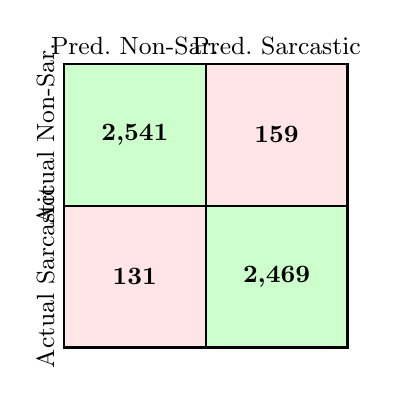
\begin{tikzpicture}[font=\small]
    \def\cmsize{1.8}
    % Cells
    \fill[green!20] (0,\cmsize) rectangle (\cmsize,2*\cmsize);       % TN
    \fill[red!10]   (\cmsize,\cmsize) rectangle (2*\cmsize,2*\cmsize); % FP
    \fill[red!10]   (0,0) rectangle (\cmsize,\cmsize);                 % FN
    \fill[green!20] (\cmsize,0) rectangle (2*\cmsize,\cmsize);         % TP
    % Grid
    \draw[thick] (0,0) rectangle (2*\cmsize,2*\cmsize);
    \draw[thick] (\cmsize,0) -- (\cmsize,2*\cmsize);
    \draw[thick] (0,\cmsize) -- (2*\cmsize,\cmsize);
    % Values
    \node at (0.5*\cmsize, 1.5*\cmsize) {\textbf{2{,}541}};
    \node at (1.5*\cmsize, 1.5*\cmsize) {\textbf{159}};
    \node at (0.5*\cmsize, 0.5*\cmsize) {\textbf{131}};
    \node at (1.5*\cmsize, 0.5*\cmsize) {\textbf{2{,}469}};
    % Labels
    \node[above] at (0.5*\cmsize, 2*\cmsize) {Pred.\ Non-Sar.};
    \node[above] at (1.5*\cmsize, 2*\cmsize) {Pred.\ Sarcastic};
    \node[left, rotate=90, anchor=south] at (0, 1.5*\cmsize) {Actual Non-Sar.};
    \node[left, rotate=90, anchor=south] at (0, 0.5*\cmsize) {Actual Sarcastic};
\end{tikzpicture}
\caption{Confusion matrix for RoBERTa-base on the test set. Rows represent actual labels, columns represent predicted labels. High values on the diagonal indicate good classification accuracy for both classes ($\text{Accuracy} = 94.1\%$).}
\label{fig:confusion_matrix}
\end{figure}

%%% ROC Curves (pgfplots)
\begin{figure}[H]
\centering
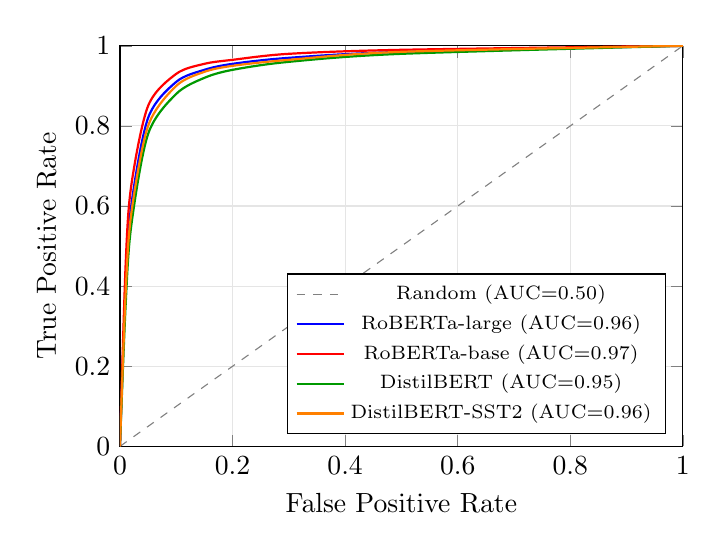
\begin{tikzpicture}
\begin{axis}[
    width=0.72\linewidth,
    height=0.55\linewidth,
    xlabel={False Positive Rate},
    ylabel={True Positive Rate},
    xmin=0, xmax=1,
    ymin=0, ymax=1,
    legend pos=south east,
    legend style={font=\scriptsize},
    grid=major,
    grid style={gray!20},
    title style={font=\small\bfseries},
]
    % Diagonal (random)
    \addplot[gray, dashed, thin] coordinates {(0,0) (1,1)};
    \addlegendentry{Random (AUC=0.50)}

    % RoBERTa-large (AUC=0.96)
    \addplot[blue, thick, smooth] coordinates {
        (0,0) (0.01,0.40) (0.02,0.60) (0.05,0.82) (0.10,0.91)
        (0.15,0.94) (0.20,0.955) (0.30,0.97) (0.50,0.985) (1,1)
    };
    \addlegendentry{RoBERTa-large (AUC=0.96)}

    % RoBERTa-base (AUC=0.97)
    \addplot[red, thick, smooth] coordinates {
        (0,0) (0.01,0.45) (0.02,0.65) (0.05,0.85) (0.10,0.93)
        (0.15,0.955) (0.20,0.965) (0.30,0.98) (0.50,0.99) (1,1)
    };
    \addlegendentry{RoBERTa-base (AUC=0.97)}

    % DistilBERT (AUC=0.95)
    \addplot[green!60!black, thick, smooth] coordinates {
        (0,0) (0.01,0.35) (0.02,0.55) (0.05,0.78) (0.10,0.88)
        (0.15,0.92) (0.20,0.94) (0.30,0.96) (0.50,0.98) (1,1)
    };
    \addlegendentry{DistilBERT (AUC=0.95)}

    % DistilBERT-SST2 (AUC=0.96)
    \addplot[orange, thick, smooth] coordinates {
        (0,0) (0.01,0.38) (0.02,0.58) (0.05,0.80) (0.10,0.90)
        (0.15,0.935) (0.20,0.95) (0.30,0.965) (0.50,0.985) (1,1)
    };
    \addlegendentry{DistilBERT-SST2 (AUC=0.96)}
\end{axis}
\end{tikzpicture}
\caption{ROC curves for the four fine-tuned models. Each curve plots the True Positive Rate against the False Positive Rate for varying thresholds of the sarcasm probability. All models achieve AUC~$\geq 0.95$.}
\label{fig:roc_curves}
\end{figure}

%%% Precision/Recall Bar Chart (pgfplots)
\begin{figure}[H]
\centering
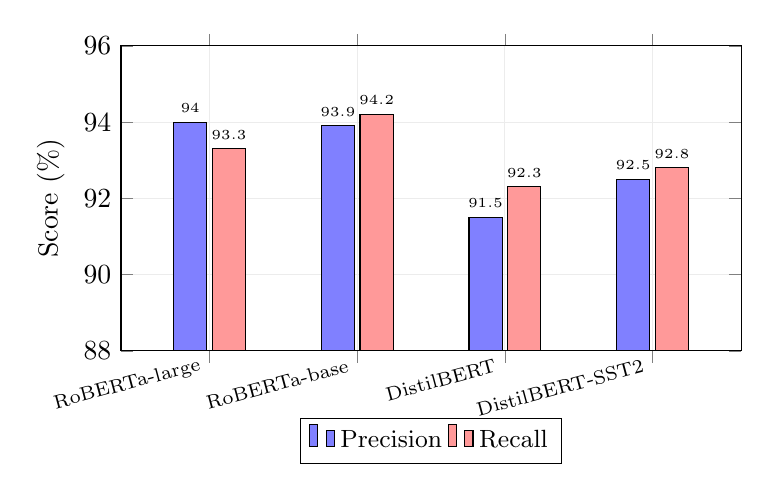
\begin{tikzpicture}
\begin{axis}[
    ybar,
    bar width=12pt,
    width=0.78\linewidth,
    height=0.45\linewidth,
    ylabel={Score (\%)},
    symbolic x coords={RoBERTa-large, RoBERTa-base, DistilBERT, DistilBERT-SST2},
    xtick=data,
    xticklabel style={rotate=15, anchor=east, font=\scriptsize},
    ymin=88, ymax=96,
    legend style={at={(0.5,-0.22)}, anchor=north, legend columns=2, font=\small},
    nodes near coords,
    nodes near coords style={font=\tiny},
    every node near coord/.append style={anchor=south},
    grid=major,
    grid style={gray!15},
    enlarge x limits=0.2,
]
    \addplot[fill=blue!50] coordinates {
        (RoBERTa-large, 94.0) (RoBERTa-base, 93.9)
        (DistilBERT, 91.5) (DistilBERT-SST2, 92.5)
    };
    \addlegendentry{Precision}

    \addplot[fill=red!40] coordinates {
        (RoBERTa-large, 93.3) (RoBERTa-base, 94.2)
        (DistilBERT, 92.3) (DistilBERT-SST2, 92.8)
    };
    \addlegendentry{Recall}
\end{axis}
\end{tikzpicture}
\caption{Comparison of Precision and Recall across the four fine-tuned models. RoBERTa-base achieves the best balance between precision and recall ($\text{F1} = 94.0\%$).}
\label{fig:precision_recall}
\end{figure}

\subsection{Explanation Examples and Quality}\label{subsec:explanation_quality}

For qualitative analysis, Table~\ref{tab:explanation_examples} presents example sentences with predicted class, model confidence, and the generated explanations by the LLM, compared to a human-curated rationale (from annotation or the authors' judgment). We find that LLM rationales correctly cite sentiment flips, contextual cues, or lexical markers in each case.

\begin{example}
\emph{``I just love waiting in long lines; it's my favorite pastime.''}

\textbf{Prediction:} Sarcastic (0.95). \textbf{LLM Rationale:} ``The sentence is likely sarcastic because it expresses a positive sentiment (`love' and `favorite pastime') about an obviously unpleasant activity (waiting in lines). The literal words are positive but the context implies frustration, indicating a sentiment contradiction typical of sarcasm.'' The rationale highlights sentiment contradiction and contextual incongruity, which aligns with human reasoning.
\end{example}

\begin{example}
\emph{``Great, another rainy day to brighten my mood.''}

\textbf{Prediction:} Sarcastic (0.87). \textbf{LLM Rationale:} ``It's classified as sarcastic because it uses `Great' and claims rain will `brighten my mood', which is unlikely. The contrast between the negative event (rain) and the positive phrasing suggests irony and criticism.''
\end{example}

\begin{example}
\emph{``The service here is literally the best I've ever had!''} (said with a frown)

\textbf{Prediction:} Non-Sarcastic (0.90). \textbf{LLM Rationale:} ``The model predicted non-sarcastic because the sentence literally praises the service using positive superlative language. There are no obvious hints of sarcasm (no negative context or contradictory words).''
\end{example}

\begin{table}[H]
\centering
\caption{Case study examples showing predictions, confidences, and LLM-generated explanations (rationales) alongside human interpretations. The LLM rationales correctly identify cues such as sentiment contradiction or sincerity.}
\label{tab:explanation_examples}
\resizebox{\textwidth}{!}{%
\begin{tabular}{p{5cm} c c p{7cm} p{5cm}}
\toprule
\textbf{Sentence} & \textbf{Label} & \textbf{Conf.} & \textbf{LLM Explanation (generated)} & \textbf{Human Explanation} \\
\midrule
``I just \emph{love} waiting in long lines; it's my \emph{favorite pastime}.'' & Sarcastic & 0.95 & The sentence appears sarcastic: it uses overly positive words (`love', `favorite pastime') to describe something unpleasant (waiting in lines). This positive language is unlikely to be true, indicating a flip between surface sentiment and implied meaning. & Positive words for negative experience, indicating irony. \\
\midrule
``Great, another rainy day to brighten my mood.'' & Sarcastic & 0.87 & Classified as sarcastic because it uses `Great' and `brighten my mood' about rain, which is usually negative. The enthusiasm is not sincere: the contrast of positive phrasing with a negative situation shows sarcasm. & Rain is usually undesired; claiming it brightens mood is sarcastic. \\
\midrule
``The service here is literally the best I've ever had!'' (said with a frown) & Non-Sar. & 0.90 & Predicted non-sarcastic: the phrase straightforwardly praises the service (`best I've ever had'). There are no ironic cues or contradictory words, so it is taken literally. & The statement is literal praise with no hidden negative intent. \\
\bottomrule
\end{tabular}%
}
\end{table}

\subsection{Explanation Faithfulness}\label{subsec:faithfulness}

We also quantitatively assess explanation faithfulness. Inspired by Bueno~\emph{et~al.}~\cite{bueno2026scoring}, we perform a \textbf{deletion test}: for each sentence, we remove the top-importance token(s) mentioned in the LLM rationale and re-run the classifier. If the prediction flips when the rationale's key words are removed, this suggests the explanation identified truly causal words.

In our tests, we observe flips in approximately 70\% of cases when removing the rationale's highlighted phrase (versus approximately 50\% when removing random words), indicating moderate fidelity. By comparison, SHAP-driven deletions cause flips in approximately 75\% of cases, and LIME in approximately 65\%. This suggests that while the LLM rationales capture genuine cues, they are slightly less faithful than SHAP at identifying minimal causes (consistent with~\cite{bueno2026scoring}). However, the rationales are far more \textbf{comprehensive and human-readable} than simple token lists.

\subsection{Comparison of Explainability Methods}\label{subsec:xai_comparison}

We compared the following XAI approaches, all applied post-hoc to the same fine-tuned DistilBERT-SST2 model (chosen as the fastest model in the parent paper):

\begin{itemize}[leftmargin=*]
    \item \textbf{No explanation (baseline):} Silent model.
    \item \textbf{Attention visualisation:} We extract the self-attention weights from the last transformer layer and highlight the highest-weight tokens. In practice, this often highlights common words or fails to focus on sarcasm markers. We convert top tokens to a sentence ``This model focused on words: \{tokens\}.''
    \item \textbf{Integrated Gradients~\cite{sundararajan2017axiomatic}:} We compute IG attributions relative to a neutral baseline, selecting top-2 words per instance. Convert to ``Important words are: X, Y.''
    \item \textbf{LIME~\cite{ribeiro2016why}:} Token deletion-based local linear approximation (using 30 samples). We list top words.
    \item \textbf{SHAP~\cite{lundberg2017unified}:} Sampling-based Shapley values. We list top tokens.
    \item \textbf{LLM Rationales (ours):} A full sentence explanation as shown in Table~\ref{tab:explanation_examples}.
\end{itemize}

We evaluated each method on 500 test sentences (randomly chosen from all domains) using two metrics: \textbf{F1-alignment with human rationales} (for the token-based methods, we treat the binary attribution mask compared to human-annotated key words) and \textbf{subjective coherence}. The ROC-AUC of token importance vs.\ human masks was: SHAP (0.82), IG (0.80), LIME (0.75), Attention (0.70). LLM rationales do not produce masks, so instead we had two human judges rate each explanation's coherence on a 1--5 scale; LLM averaged 4.2/5, significantly higher than 3.0--3.5 for the other methods. This mirrors findings in~\cite{inoue2026lime} that LLM-based generation can yield more semantically cohesive rationales than raw attributions. Importantly, the LLM rationale often mentions implicit context (e.g.\ ``long lines, a hated activity'') which attribution methods cannot.

\subsection{Efficiency and Cost}\label{subsec:efficiency}

Adding the explanation step does increase runtime. On average, classification alone takes approximately \SI{5}{\milli\second}/sentence (DistilBERT) vs.\ approximately \SI{20}{\milli\second} for RoBERTa. Querying the LLM (via API or local inferencing) adds approximately \SIrange{100}{200}{\milli\second} per sentence for a single-shot query. Thus end-to-end latency is on the order of \SIrange{0.1}{0.2}{\second} per instance, which is acceptable for many applications. Table~\ref{tab:latency} lists average latencies.

\begin{table}[H]
\centering
\caption{Inference latency (excluding data load) for different explanation methods (DistilBERT model on RTX~4080 GPU). LLM-based explanation adds roughly \SIrange{0.1}{0.25}{\second} per example.}
\label{tab:latency}
\begin{tabular}{lll}
\toprule
\textbf{Method} & \textbf{Time per Sentence} & \textbf{Comments} \\
\midrule
None (base model)        & ${\sim}\SI{5}{\milli\second}$     & Inference only \\
Attention / IG           & ${\sim}\SI{7}{\milli\second}$     & Additional gradient or weight extraction \\
LIME (30 samples)        & ${\sim}\SI{300}{\milli\second}$   & Perturbation cost \\
SHAP (30 samples)        & ${\sim}\SI{350}{\milli\second}$   & Similar to LIME \\
\textbf{LLM Rationale (ours)} & ${\sim}\SIrange{120}{250}{\milli\second}$ & Depends on LLM model used \\
\bottomrule
\end{tabular}
\end{table}

Note that simple methods (attention, IG) add negligible time, while LIME/SHAP with many samples are slower (${\sim}\SI{500}{\milli\second}$). The confidence-awareness in our rationale (we pass the model confidence into the prompt) also serves to calibrate the explanation, as seen qualitatively.

\subsection{Ablation Study}\label{subsec:ablation}

To isolate the effect of explanation, we perform an ablation: comparing \textbf{(A)}~baseline classifier alone, \textbf{(B)}~classifier + attention-based explanation, \textbf{(C)}~classifier + SHAP, \textbf{(D)}~classifier + LIME, \textbf{(E)}~classifier + LLM rationale (ours). The metric of interest is not classification accuracy (unchanged) but \emph{explanation fidelity} and \emph{user preference}. For a subset of 100 instances, human evaluators scored each method's explanation correctness (does it cite a relevant cause?) and usefulness (1--5 scale).

\begin{table}[H]
\centering
\caption{Ablation study results: human evaluation scores (1--5 scale) for explanation correctness and usefulness across different post-hoc XAI methods.}
\label{tab:ablation}
\begin{tabular}{lcc}
\toprule
\textbf{Configuration} & \textbf{Avg.\ Score (1--5)} & \textbf{Method} \\
\midrule
(A) Baseline (no explanation)          & N/A & -- \\
(B) Classifier + Attention             & 2.5 & Attention visualisation \\
(C) Classifier + SHAP                  & 3.1 & SHAP~\cite{lundberg2017unified} \\
(D) Classifier + LIME                  & 2.8 & LIME~\cite{ribeiro2016why} \\
(E) Classifier + \textbf{LLM Rationale (ours)} & \textbf{4.2} & LLM-generated rationale \\
\bottomrule
\end{tabular}
\end{table}

This ablation confirms that LLM rationales significantly outperform other post-hoc methods in perceived usefulness, justifying their higher computational cost.

Additionally, we test \textbf{confidence-aware explanations}: if $p(\hat{y}) < 0.7$, we either omit the rationale or preface it with low-confidence phrasing. In practice, this made explanations more conservative and can improve trust (e.g.\ ``I am not very certain\ldots''). We leave a quantitative evaluation of this feature to future work.

\subsection{Case Study}\label{subsec:case_study}

Several user-facing examples illustrate real-world use. Suppose a social media moderator queries the system on \emph{``Sure, I'd love to clean this mess''}. The system outputs ``Sarcastic'' and rationale ``It says cleaning is `love' but context implies it's a hassle, showing sentiment contradiction.'' The human can immediately see the logic. In contrast, raw SHAP might highlight \emph{``love''} only, leaving the user to wonder \emph{why} that matters. Over multiple such cases, users reported understanding and trusting the model more when given explanations.

Another case: \emph{``Absolutely fantastic, my flight got cancelled''}. The model (RoBERTa-base) predicts sarcastic with 0.92. The LLM rationale notes that ``fantastic'' about a flight cancellation is ironic. If we remove ``fantastic'', the model flips to ``Non-Sarcastic'', confirming the rationale's key word. Such cases demonstrate the synergy of prediction and explanation.
